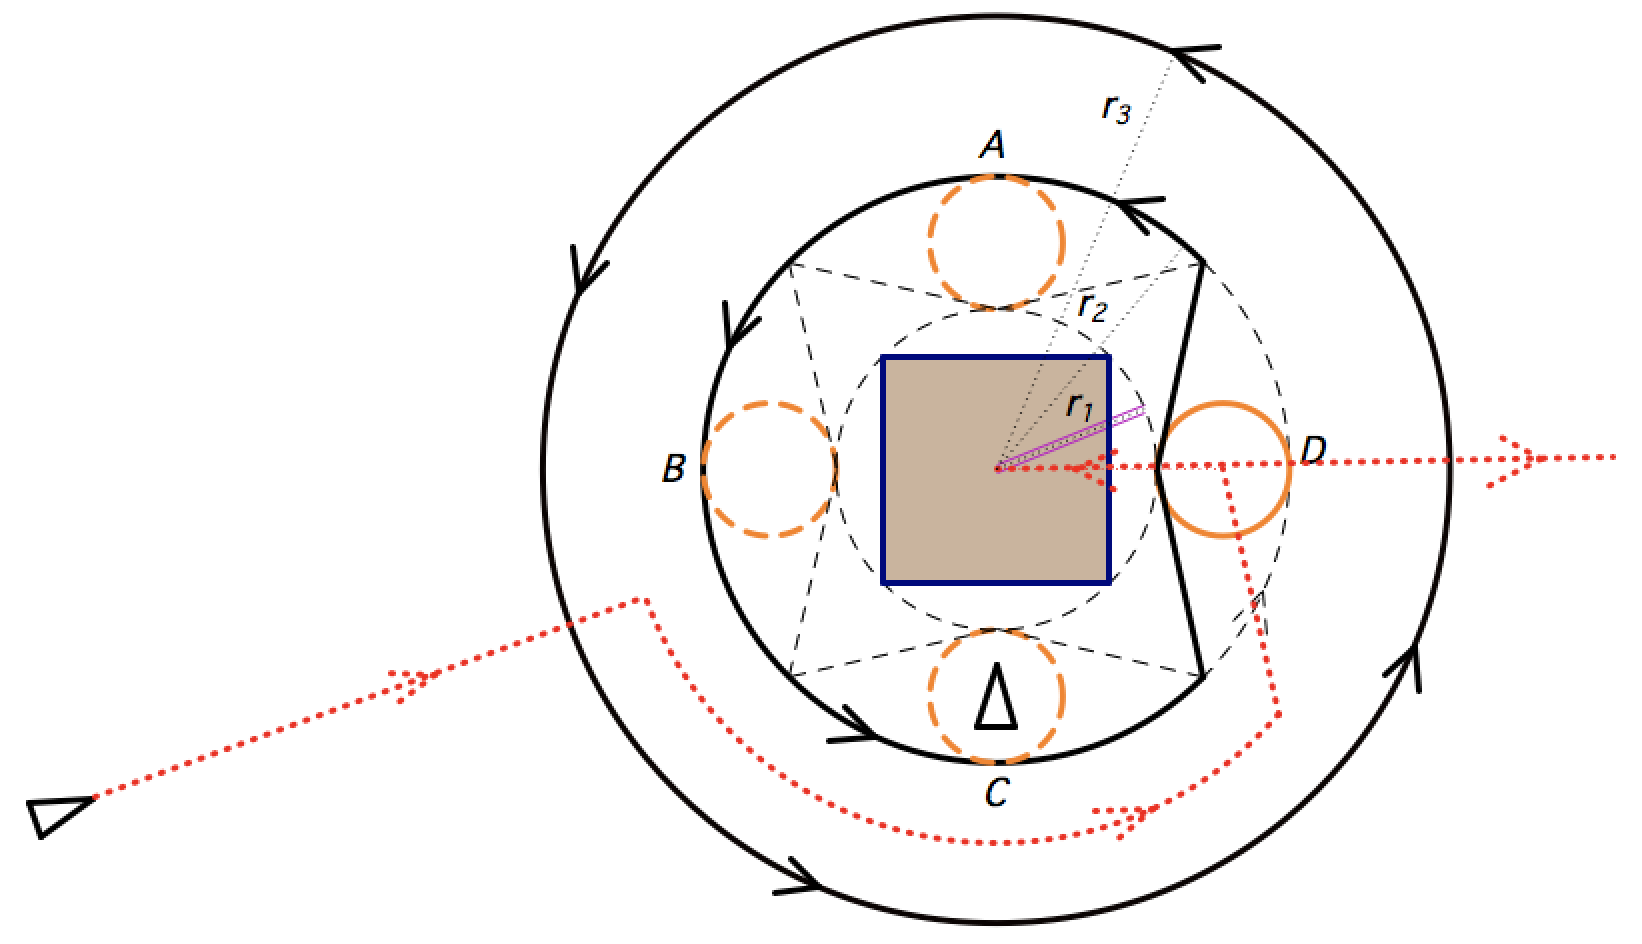
\includegraphics[scale=0.3]{driveway}

Agent localization can be broken down into two parts: 1) static initialization, and 2) dynamic refactoring.

\begin{algorithm} 
	\caption{\textit{Static Initialization}: create reference anchor node based on collective agent position.}
	\label{alg:init}
	\begin{algorithmic}[1]
		\renewcommand{\algorithmicrequire}{\textbf{Input:}}
		\renewcommand{\algorithmicensure}{\textbf{Output:}}
		\REQUIRE $X_p:$ the perceived agent position.
		\ENSURE  $X_A$: the position of the reference anchor node.
		
		\RETURN $S, V$
	\end{algorithmic}
\end{algorithm}

After initialization, localization aims to improve the percieved location of the agent by correcting the recorded pose by a dynamic $x$ and $y$ offset. These offsets can be model by the equations,

\begin{equation}
	(x, y) = w \cdot ((x, y)_c - (x, y)_p) + u \cdot (x, y)_g - (x, y)_c) + v \cdot (cos/sin)(\theta) 
\end{equation}

where $(x, y)_c$ and $(x, y)_p$ are the current and previously recorded GPS locations, $(x, y)_g$ is the goal agent location and $\theta$ is the current heading. The weights applied to the relative change in position $w, u,$ and $v$ can then be model by the piece wise functions,

\begin{equation}
	w = 
	\begin{cases}
		1 & \mathcal{D_A}} < 0.1 \\
		e^{-(x, y)} & \text{otherwise}
	\end{cases}
\end{equation}

\begin{equation}
	u = 
	\begin{cases}
		1 & \mathcal{D_G} < 0.05 \\
		\frac{1}{1 + (x, y)} & \text{otherwise}
	\end{cases}
\end{equation}

\begin{equation}
	v = 
	\begin{cases}
		0 & \frac{d(x, y)}{dt} < 0.01 \\
		(\frac{d(x, y)}{dt})^2 & \text{otherwise}
	\end{cases}
\end{equation}

such that $\mathcal{D_A}$ is the distance from the anchor node, $\mathcal{D_G}$ is the distance to the goal location, and $\frac{d(x,y)}{dt}$ is the linear velocity of the agent. 